\documentclass[11pt, a4paper]{article}

% Fonts and Encoding
\usepackage[utf8]{inputenc}
\usepackage[T1]{fontenc}

% Math and Symbols
\usepackage{amsmath, amssymb, amsthm, amsfonts, mathrsfs, mathtools}

% Layout and Geometry
\usepackage{geometry}
\geometry{a4paper, margin=1in}

% Formatting and Graphics
\usepackage{graphicx, xcolor, enumitem, booktabs, array, tabularx}

% TikZ for Illustrations
\usepackage{tikz}
\usetikzlibrary{arrows.meta, positioning, shapes.geometric, calc, backgrounds}

% Clickable Links and TOC
\usepackage{hyperref}
\hypersetup{
    colorlinks=true,
    linkcolor=blue,
    filecolor=magenta,      
    urlcolor=cyan,
    pdftitle={Advanced Mathematics Topic},
}

% Theorem Environments
\newtheorem{theorem}{Theorem}[section]
\newtheorem{lemma}[theorem]{Lemma}
\newtheorem{proposition}[theorem]{Proposition}
\newtheorem{corollary}[theorem]{Corollary}
\theoremstyle{definition}
\newtheorem{definition}{Definition}[section]
\newtheorem{axiom}{Axiom}[section]
\newtheorem{example}{Example}[section]
\theoremstyle{remark}
\newtheorem{remark}{Remark}[section]

% Custom Commands
\newcommand{\R}{\mathbb{R}}
\newcommand{\N}{\mathbb{N}}
\newcommand{\Z}{\mathbb{Z}}
\newcommand{\Q}{\mathbb{Q}}
\newcommand{\E}{\mathbb{E}}
\newcommand{\Prob}{\mathbb{P}}
\newcommand{\F}{\mathcal{F}}

\title{\textbf{Expectations of Discontinuous Functions and Mixed Probability Distributions}}
\author{Tashfeen Omran}
\date{\today}

\begin{document}

\maketitle
\tableofcontents
\newpage

\section{Part 1: Comprehensive Introduction, Context, and Prerequisites}

\subsection{Core Concepts \& Axioms}
In standard introductory probability, random variables are typically bifurcated into two mutually exclusive categories: \textit{discrete} (taking values in a countable set with a probability mass function) and \textit{continuous} (taking values in an uncountable set with a probability density function). However, this dichotomy is mathematically incomplete. 

In advanced probability theory, a random variable $Y$ is simply a measurable function from a probability space $(\Omega, \F, \Prob)$ to the measurable space $(\R, \mathcal{B}(\R))$, where $\mathcal{B}(\R)$ is the Borel $\sigma$-algebra. The distribution of $Y$ is completely characterized by its Cumulative Distribution Function (CDF), defined as $F(y) = \Prob(Y \le y)$. 

A \textbf{mixed probability distribution} arises when the CDF $F(y)$ is neither a step function (purely discrete) nor an absolutely continuous function (purely continuous). Instead, $F(y)$ contains both continuous intervals where $F'(y) > 0$ and isolated points of discontinuity (jumps) where $\Prob(Y = y) > 0$. 

By a simplified version of the \textbf{Lebesgue Decomposition Theorem}, any practical CDF can be uniquely expressed as a convex combination of a discrete CDF and a continuous CDF:
\[ F(y) = c_1 F_1(y) + c_2 F_2(y) \]
where:
\begin{itemize}
    \item $F_1(y)$ is a step distribution function (the discrete component).
    \item $F_2(y)$ is an absolutely continuous distribution function (the continuous component).
    \item $c_1, c_2 \ge 0$ such that $c_1 + c_2 = 1$. Here, $c_1$ represents the total probability mass concentrated at the discrete jump points.
\end{itemize}

\subsection{Intuition and Set-Theoretic Foundations}
Intuitively, a mixed distribution models a population that is a \textit{mixture} of two distinct sub-populations. Imagine an insurance portfolio: a large fraction of clients ($c_1$) will file zero claims (a discrete mass at $Y = 0$), while the remaining clients ($c_2$) will file claims of varying, continuous amounts (a continuous distribution for $Y > 0$). 

Set-theoretically, we are partitioning the sample space $\Omega$ into two disjoint measurable sets, $A$ and $A^c$, where $\Prob(A) = c_1$ and $\Prob(A^c) = c_2$. Conditional on $\omega \in A$, the random variable $Y(\omega)$ behaves discretely. Conditional on $\omega \in A^c$, $Y(\omega)$ behaves continuously. The Law of Total Probability stitches these two spaces together to form the mixed CDF.

\subsection{Historical Context and Motivation}
Before the 20th century, mathematicians struggled to unify the theories of discrete summation and continuous integration. The foundational crisis was resolved in 1902 by Henri Lebesgue, who introduced Measure Theory. Lebesgue integration provided a unified framework where both sums (using the counting measure) and integrals (using the Lebesgue measure) were treated as identical mathematical objects. This allowed statisticians to formalize mixed distributions without relying on ad-hoc piecewise notation, paving the way for modern stochastic calculus and survival analysis.

\subsection{Key Theorems and Formulas}
\begin{theorem}[Expectation of a Mixed Distribution]
Let $Y$ have a mixed distribution $F(y) = c_1 F_1(y) + c_2 F_2(y)$. Let $X_1$ be a discrete random variable with CDF $F_1(y)$ and $X_2$ be a continuous random variable with CDF $F_2(y)$. For any measurable function $g$, the expected value is given by:
\[ \E[g(Y)] = c_1 \E[g(X_1)] + c_2 \E[g(X_2)] \]
provided the expectations exist.
\end{theorem}

\subsection{Prerequisites}
To master this topic, one must be proficient in:
\begin{itemize}
    \item \textbf{Calculus:} Integration by parts, improper integrals, and differentiating piecewise functions.
    \item \textbf{Probability Foundations:} The Law of the Unconscious Statistician (LOTUS), properties of Cumulative Distribution Functions (right-continuity, limits at infinity).
    \item \textbf{Algebraic Manipulation:} Solving systems of equations to find mixing weights $c_1$ and $c_2$.
\end{itemize}

\newpage
\section{Part 2: Detailed Homework Solutions}

\subsection{Problem 4.155: Discontinuous Function of a Continuous Variable}
\textbf{Problem Statement:} A builder orders supplies with a waiting time $Y \sim \text{Uniform}(1, 4)$ days. If the delay is up to 2 days, the cost is fixed at $\$100$. After 2 days, the cost is $\$100$ plus $\$20$ per day (prorated) for each additional day. Find the expected value of the builder's cost.

\begin{proof}[Solution via Direct Computation (LOTUS)]
\textbf{Step 1: Define the random variable and its density.} \\
The waiting time $Y$ is uniformly distributed on $[1, 4]$. The probability density function (PDF) is:
\[ f(y) = \begin{cases} \frac{1}{4 - 1} = \frac{1}{3}, & 1 \le y \le 4 \\ 0, & \text{otherwise} \end{cases} \]

\textbf{Step 2: Formulate the cost function $C(Y)$.} \\
The cost is a discontinuous piecewise function of $Y$:
\[ C(Y) = \begin{cases} 100, & 1 \le Y \le 2 \\ 100 + 20(Y - 2), & 2 < Y \le 4 \end{cases} \]
Simplifying the second branch: $100 + 20Y - 40 = 60 + 20Y$.

\textbf{Step 3: Apply the Law of the Unconscious Statistician (LOTUS).} \\
The expected cost is $\E[C(Y)] = \int_{-\infty}^{\infty} C(y) f(y) \, dy$. We split the integral at the point of discontinuity $y = 2$:
\begin{align*}
\E[C(Y)] &= \int_{1}^{2} 100 \left(\frac{1}{3}\right) \, dy + \int_{2}^{4} (60 + 20y) \left(\frac{1}{3}\right) \, dy \\
&= \frac{100}{3} \Big[ y \Big]_{1}^{2} + \frac{1}{3} \int_{2}^{4} (60 + 20y) \, dy \\
&= \frac{100}{3}(2 - 1) + \frac{1}{3} \Big[ 60y + 10y^2 \Big]_{2}^{4}
\end{align*}

\textbf{Step 4: Evaluate the definite integrals.} \\
Evaluate the bounds for the second term:
\[ \Big[ 60(4) + 10(4)^2 \Big] - \Big[ 60(2) + 10(2)^2 \Big] = (240 + 160) - (120 + 40) = 400 - 160 = 240 \]
Substitute this back into the expectation equation:
\[ \E[C(Y)] = \frac{100}{3} + \frac{1}{3}(240) = \frac{340}{3} \approx 113.33 \]

\textbf{Conclusion:} The expected value of the builder's cost is $\$113.33$. $\blacksquare$
\end{proof}

\subsection{Problem 4.157: Censored Distribution (Mixed RV)}
\textbf{Problem Statement:} The life length $Y$ of a component has an exponential density with a mean of 100 hours. The component is replaced at failure or at age 200 hours, whichever comes first. Let $X$ be the length of time the component is in use. 
(a) Find the distribution function for $X$. 
(b) Find $\E[X]$.

\begin{proof}[Solution via Measure-Theoretic Truncation]
\textbf{Part (a): Distribution Function of $X$} \\
\textbf{Step 1: Define the underlying variable.} \\
$Y \sim \text{Exponential}(\beta = 100)$. The density is $f_Y(y) = \frac{1}{100}e^{-y/100}$ for $y > 0$. The CDF is $F_Y(y) = 1 - e^{-y/100}$.

\textbf{Step 2: Define the transformation.} \\
The time in use is $X = \min(Y, 200)$. This is a classic right-censored variable.

\textbf{Step 3: Construct the CDF $F_X(x) = \Prob(X \le x)$.} \\
\begin{itemize}
    \item For $x < 0$: $F_X(x) = 0$.
    \item For $0 \le x < 200$: The event $\{X \le x\}$ is identical to $\{Y \le x\}$. Thus, $F_X(x) = 1 - e^{-x/100}$.
    \item For $x \ge 200$: Since the component is always replaced by 200 hours, $X$ can never exceed 200. Thus, $\Prob(X \le x) = 1$.
\end{itemize}
\[ F_X(x) = \begin{cases} 0, & x < 0 \\ 1 - e^{-x/100}, & 0 \le x < 200 \\ 1, & x \ge 200 \end{cases} \]

\textbf{Part (b): Expected Value of $X$} \\
\textbf{Step 4: Identify the mixed components.} \\
$X$ has a continuous distribution on $[0, 200)$ and a discrete point mass at $x = 200$. The probability of the discrete mass is:
\[ \Prob(X = 200) = \Prob(Y \ge 200) = e^{-200/100} = e^{-2} \]

\textbf{Step 5: Calculate Expectation.} \\
Using the definition of expectation for a mixed variable:
\[ \E[X] = \int_{0}^{200} x f_Y(x) \, dx + 200 \cdot \Prob(X = 200) \]
\[ \E[X] = \int_{0}^{200} x \left(\frac{1}{100}e^{-x/100}\right) \, dx + 200e^{-2} \]
We use integration by parts for the integral. Let $u = x \implies du = dx$, and $dv = \frac{1}{100}e^{-x/100}dx \implies v = -e^{-x/100}$.
\begin{align*}
\int_{0}^{200} x \left(\frac{1}{100}e^{-x/100}\right) \, dx &= \Big[ -x e^{-x/100} \Big]_{0}^{200} - \int_{0}^{200} -e^{-x/100} \, dx \\
&= -200e^{-2} - 0 + \Big[ -100e^{-x/100} \Big]_{0}^{200} \\
&= -200e^{-2} - 100e^{-2} + 100 = 100 - 300e^{-2}
\end{align*}
Adding the discrete component back:
\[ \E[X] = (100 - 300e^{-2}) + 200e^{-2} = 100 - 100e^{-2} = 100(1 - e^{-2}) \]

\textbf{Conclusion:} The expected time in use is $100(1 - e^{-2})$ hours. $\blacksquare$
\end{proof}

\subsection{Problem 4.159: Decomposing a Mixed CDF}
\textbf{Problem Statement:} A random variable $Y$ has the distribution function:
\[ F(y) = \begin{cases} 0, & y < 0 \\ y^2 + 0.1, & 0 \le y < 0.5 \\ y, & 0.5 \le y < 1 \\ 1, & y \ge 1 \end{cases} \]
(a) Give $F_1(y)$ and $F_2(y)$, the discrete and continuous components. 
(b) Write $F(y) = c_1 F_1(y) + c_2 F_2(y)$. 
(c) Find the expected value and variance of $Y$.

\begin{proof}[Solution via CDF Decomposition]
\textbf{Part (a) \& (b): Decomposition} \\
\textbf{Step 1: Locate the discrete jumps.} \\
A jump occurs where $\lim_{y \to a^-} F(y) \neq F(a)$.
\begin{itemize}
    \item At $y = 0$: $F(0) - F(0^-) = (0^2 + 0.1) - 0 = 0.1$.
    \item At $y = 0.5$: $F(0.5) - F(0.5^-) = 0.5 - (0.5^2 + 0.1) = 0.5 - 0.35 = 0.15$.
    \item At $y = 1$: $F(1) - F(1^-) = 1 - 1 = 0$ (No jump).
\end{itemize}
The total discrete probability mass is $c_1 = 0.1 + 0.15 = 0.25$. Consequently, the continuous weight is $c_2 = 1 - c_1 = 0.75$.

\textbf{Step 2: Construct the discrete CDF $F_1(y)$.} \\
$F_1(y)$ is formed by accumulating the normalized jump probabilities (dividing by $c_1 = 0.25$):
\[ F_1(y) = \begin{cases} 0, & y < 0 \\ \frac{0.1}{0.25} = 0.4, & 0 \le y < 0.5 \\ \frac{0.1 + 0.15}{0.25} = 1, & y \ge 0.5 \end{cases} \]

\textbf{Step 3: Construct the continuous CDF $F_2(y)$.} \\
Using the relation $F_2(y) = \frac{F(y) - c_1 F_1(y)}{c_2}$:
\begin{itemize}
    \item For $0 \le y < 0.5$: $F_2(y) = \frac{(y^2 + 0.1) - 0.25(0.4)}{0.75} = \frac{y^2}{0.75} = \frac{4}{3}y^2$.
    \item For $0.5 \le y < 1$: $F_2(y) = \frac{y - 0.25(1)}{0.75} = \frac{y - 0.25}{0.75} = \frac{4}{3}y - \frac{1}{3}$.
    \item For $y \ge 1$: $F_2(y) = \frac{1 - 0.25}{0.75} = 1$.
\end{itemize}
Thus, $F(y) = 0.25 F_1(y) + 0.75 F_2(y)$.

\textbf{Part (c): Expectation and Variance} \\
\textbf{Step 4: Calculate moments of the discrete component $X_1$.} \\
$X_1$ takes value $0$ with probability $0.4$, and $0.5$ with probability $0.6$.
\[ \E[X_1] = 0(0.4) + 0.5(0.6) = 0.3 \]
\[ \E[X_1^2] = 0^2(0.4) + 0.5^2(0.6) = 0.25(0.6) = 0.15 \]

\textbf{Step 5: Calculate moments of the continuous component $X_2$.} \\
The density $f_2(y) = F_2'(y)$ is:
\[ f_2(y) = \begin{cases} \frac{8}{3}y, & 0 \le y < 0.5 \\ \frac{4}{3}, & 0.5 \le y < 1 \\ 0, & \text{otherwise} \end{cases} \]
\[ \E[X_2] = \int_{0}^{0.5} y\left(\frac{8}{3}y\right) dy + \int_{0.5}^{1} y\left(\frac{4}{3}\right) dy = \Big[ \frac{8}{9}y^3 \Big]_{0}^{0.5} + \Big[ \frac{2}{3}y^2 \Big]_{0.5}^{1} = \frac{8}{9}\left(\frac{1}{8}\right) + \frac{2}{3}\left(1 - \frac{1}{4}\right) = \frac{1}{9} + \frac{1}{2} = \frac{11}{18} \]
\[ \E[X_2^2] = \int_{0}^{0.5} y^2\left(\frac{8}{3}y\right) dy + \int_{0.5}^{1} y^2\left(\frac{4}{3}\right) dy = \Big[ \frac{2}{3}y^4 \Big]_{0}^{0.5} + \Big[ \frac{4}{9}y^3 \Big]_{0.5}^{1} = \frac{2}{3}\left(\frac{1}{16}\right) + \frac{4}{9}\left(\frac{7}{8}\right) = \frac{1}{24} + \frac{7}{18} = \frac{31}{72} \]

\textbf{Step 6: Combine to find $\E[Y]$ and $V(Y)$.} \\
\[ \E[Y] = c_1 \E[X_1] + c_2 \E[X_2] = \frac{1}{4}\left(\frac{3}{10}\right) + \frac{3}{4}\left(\frac{11}{18}\right) = \frac{3}{40} + \frac{11}{24} = \frac{9 + 55}{120} = \frac{64}{120} = \frac{8}{15} \]
\[ \E[Y^2] = c_1 \E[X_1^2] + c_2 \E[X_2^2] = \frac{1}{4}\left(\frac{3}{20}\right) + \frac{3}{4}\left(\frac{31}{72}\right) = \frac{3}{80} + \frac{31}{96} = \frac{18 + 155}{480} = \frac{173}{480} \]
\[ V(Y) = \E[Y^2] - (\E[Y])^2 = \frac{173}{480} - \left(\frac{8}{15}\right)^2 = \frac{173}{480} - \frac{64}{225} = \frac{2595 - 2048}{7200} = \frac{547}{7200} \]

\textbf{Conclusion:} $\E[Y] = \frac{8}{15}$ and $V(Y) = \frac{547}{7200}$. $\blacksquare$
\end{proof}

\newpage
\section{Part 3: In-Depth Analysis of Problems and Techniques}

\subsection{A) Problem Types and Logical Strategies}
The problems solved above represent three distinct archetypes in advanced probability:
\begin{enumerate}
    \item \textbf{Piecewise Transformations (Problem 4.155):} The underlying random variable is strictly continuous, but the function applied to it, $g(Y)$, is discontinuous. The strategy is to partition the integral over the support of $Y$ into sub-intervals corresponding to the piecewise definitions of $g(Y)$.
    \item \textbf{Censoring and Truncation (Problem 4.157):} This occurs when a continuous process is artificially capped (e.g., a machine replaced at a specific time). The strategy is to recognize that the probability mass of the "tail" of the continuous distribution is swept up and concentrated at the truncation point, creating a discrete jump.
    \item \textbf{CDF Decomposition (Problem 4.159):} The most abstract archetype. You are given a raw mathematical function and must extract the measure-theoretic components. The strategy relies on analyzing the left-hand limits of the CDF to isolate point masses, subtracting them out, and scaling the remainder to form a valid continuous density.
\end{enumerate}

\subsection{B) Key Analytical and Logical Manipulations}
\begin{itemize}
    \item \textbf{Isolating Jumps via Limits:} In Problem 4.159, the critical logical trick was evaluating $\lim_{y \to a^-} F(y)$. Because a CDF is right-continuous by definition, any discrepancy between the left-hand limit and the actual function value $F(a)$ mathematically proves the existence of a discrete point mass (a Dirac delta function in the density).
    \item \textbf{Scaling Factors ($1/c_1$ and $1/c_2$):} When decomposing a mixed CDF, subtracting the discrete jumps leaves a function that only integrates to $c_2$, not $1$. A common analytical manipulation is dividing by $c_2$ to normalize the continuous component, ensuring $F_2(y)$ satisfies the axioms of a valid probability distribution.
    \item \textbf{Non-Linearity of Variance:} In Problem 4.159, we explicitly avoided the trap of calculating $V(Y) = c_1 V(X_1) + c_2 V(X_2)$. Variance is a quadratic operator, not a linear one. The rigorous technique is to use linearity strictly on the raw moments ($\E[Y]$ and $\E[Y^2]$) and compute the variance at the very end.
\end{itemize}

\newpage
\section{Part 4: "Cheatsheet", Visuals, and Tips for Success}

\subsection{Theorems \& Equivalences}
\begin{table}[htbp]
\centering
\renewcommand{\arraystretch}{1.5}
\begin{tabularx}{\textwidth}{@{} l X @{}}
\toprule
\textbf{Concept} & \textbf{Mathematical Formulation / Description} \\
\midrule
Mixed CDF Decomposition & $F(y) = c_1 F_1(y) + c_2 F_2(y)$, where $c_1 + c_2 = 1$. \\
Expectation (LOTUS) & $\E[g(Y)] = c_1 \E[g(X_1)] + c_2 \E[g(X_2)]$. \\
Second Moment & $\E[Y^2] = c_1 \E[X_1^2] + c_2 \E[X_2^2]$. \\
Survival Function Formula & $\E[Y] = \int_0^\infty (1 - F(y)) \, dy$ for any $Y \ge 0$. \\
\bottomrule
\end{tabularx}
\caption{Key Theorems and Equivalences}
\end{table}

\subsection{Set \& Logic Illustrations: The Mixed CDF}
The following TikZ diagram illustrates the anatomy of a mixed Cumulative Distribution Function. Notice how the function contains both smooth, differentiable curves (the continuous component) and vertical discontinuities (the discrete point masses).

\begin{center}
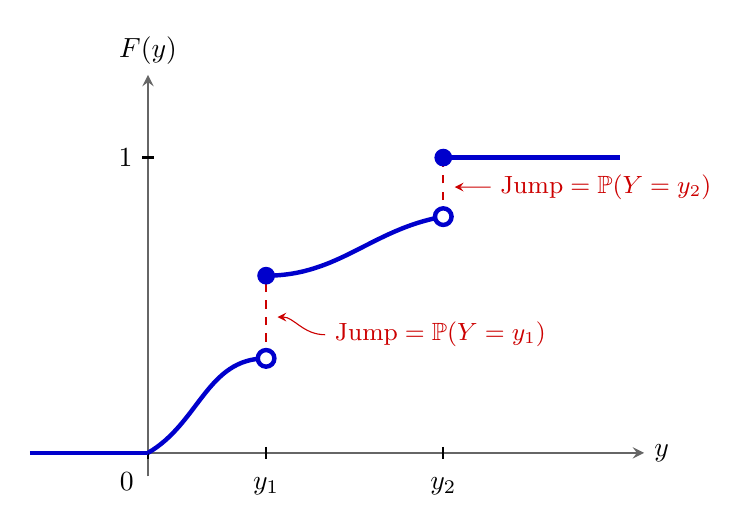
\begin{tikzpicture}[
    scale=1.5, % Global canvas scaling for maximum legibility
    >=stealth
]
    % 1. LAYER 1: Clean, Extended Axes
    \draw[->, thick, gray!80!black] (-1, 0) -- (4.2, 0) node[right, black] {$y$};
    \draw[->, thick, gray!80!black] (0, -0.2) -- (0, 3.2) node[above, black] {$F(y)$};
    
    % 2. LAYER 2: Decoupled Axis Ticks & Anchors
    \draw[thick] (-0.05, 2.5) -- (0.05, 2.5) node[left=4pt, black] {$1$};
    \draw[thick] (0,0) -- (0,-0.05) node[below left=2pt, black] {$0$};
    \draw[thick] (1, 0.05) -- (1, -0.05) node[below=3pt, black] {$y_1$};
    \draw[thick] (2.5, 0.05) -- (2.5, -0.05) node[below=3pt, black] {$y_2$};
    
    % 3. LAYER 3: CDF Function Curve Parts (Bolder lines)
    % Part 1: y < 0
    \draw[blue!80!black, ultra thick] (-1, 0) -- (0, 0);
    
    % Part 2: 0 <= y < y1
    \draw[blue!80!black, ultra thick] (0, 0) to[out=30, in=180] (1, 0.8);
    
    % Part 3: y1 <= y < y2
    \draw[blue!80!black, ultra thick] (1, 1.5) to[out=0, in=190] (2.5, 2.0);
    
    % Part 4: y >= y2
    \draw[blue!80!black, ultra thick] (2.5, 2.5) -- (4.0, 2.5);
    
    % 4. LAYER 4: Jump Discontinuities (Dashed lines and endpoint nodes)
    \draw[red!80!black, thick, dashed] (1, 0.8) -- (1, 1.5);
    \draw[red!80!black, thick, dashed] (2.5, 2.0) -- (2.5, 2.5);
    
    % Open/Closed Circle Markers (Layered carefully on top of lines)
    \filldraw[white, draw=blue!80!black, ultra thick] (1, 0.8) circle (2pt);
    \filldraw[blue!80!black] (1, 1.5) circle (2pt);
    
    \filldraw[white, draw=blue!80!black, ultra thick] (2.5, 2.0) circle (2pt);
    \filldraw[blue!80!black] (2.5, 2.5) circle (2pt);
    
    % 5. LAYER 5: Off-Axis Annotations with Precise Callouts
    % Jump 1 Callout
    \node[anchor=west, red!80!black, font=\small] (Jump1) at (1.5, 1.0) {$\text{Jump} = \mathbb{P}(Y = y_1)$};
    \draw[->, shorten >=2pt, red!80!black, thin] (Jump1.west) to[out=180, in=0] (1.05, 1.15);
    
    % Jump 2 Callout
    \node[anchor=west, red!80!black, font=\small] (Jump2) at (2.9, 2.25) {$\text{Jump} = \mathbb{P}(Y = y_2)$};
    \draw[->, shorten >=2pt, red!80!black, thin] (Jump2.west) to[out=180, in=0] (2.55, 2.25);

\end{tikzpicture}
\end{center}


\subsection{Pitfalls \& Fallacies}
\begin{table}[htbp]
\centering
\renewcommand{\arraystretch}{1.5}
\begin{tabularx}{\textwidth}{@{} l X @{}}
\toprule
\textbf{Fallacy / Pitfall} & \textbf{Explanation \& Resolution} \\
\midrule
Linearity of Variance & Assuming $V(Y) = c_1 V(X_1) + c_2 V(X_2)$. Variance is not a linear operator. You must compute $\E[Y^2]$ and $\E[Y]$ separately, then use $V(Y) = \E[Y^2] - (\E[Y])^2$. \\
Ignoring Discrete Jumps & Differentiating a mixed CDF everywhere and integrating $y f(y)$ while ignoring the point masses. The discrete jumps must be accounted for via summation. \\
Miscalculating $c_1$ & Summing the $y$-values where jumps occur instead of summing the probabilities (the magnitudes of the jumps on the y-axis). \\
\bottomrule
\end{tabularx}
\caption{Common Pitfalls and Logical Fallacies}
\end{table}

\newpage
\section{Part 5: Conceptual Synthesis and The "Big Picture"}

\subsection{A) Thematic Connections}
The central theme of this topic is \textbf{Measure-Theoretic Unification}. In early calculus, sums ($\Sigma$) and integrals ($\int$) are taught as entirely different operations. Mixed distributions force the student to realize that they are two sides of the exact same coin. By viewing probability as a measure (a function that assigns "weight" to sets), a discrete point is simply a set of size zero that happens to carry non-zero weight, while a continuous interval is a set of non-zero size where the weight is smeared smoothly. 

\subsection{B) Forward and Backward Links}
\begin{itemize}
    \item \textbf{Backward Links:} This topic extends the basic definitions of Expected Value and Cumulative Distribution Functions. It challenges the naive assumption that $F'(y)$ always yields a complete probability density function.
    \item \textbf{Forward Links:} Understanding mixed distributions is the absolute bedrock for advanced Stochastic Calculus and Measure Theory. In graduate-level probability, you will encounter the Radon-Nikodym derivative, which formalizes how to integrate with respect to mixed measures. Furthermore, in stochastic processes, this concept evolves into \textit{Jump-Diffusion models} (e.g., Lévy processes), where a particle moves continuously (Brownian motion) but occasionally experiences sudden, discrete jumps (Poisson process).
\end{itemize}

\section{Part 6: Abstract Real-World Modeling (AI, ML, \& Quant Finance)}

\subsection{A) Concrete Scenarios}
\begin{enumerate}
    \item \textbf{Quantitative Finance (Credit Risk Modeling):} When pricing corporate bonds, the time-to-default $\tau$ of a company is modeled as a mixed distribution. There is a discrete probability $p$ that the company is already insolvent at $t=0$ (revealed only upon audit), and a continuous exponential distribution for default at any time $t > 0$.
    \item \textbf{Machine Learning (Zero-Inflated Models):} In predictive modeling for e-commerce, the amount of money a user spends in a day is a mixed variable. A massive portion of users spend exactly $\$0$ (discrete mass), while paying users spend a continuous amount modeled by a Gamma or Lognormal distribution. Standard regression fails here; one must use Zero-Inflated Poisson (ZIP) or Hurdle models.
\end{enumerate}

\subsection{B) Model Problem Setup: Credit Default Pricing}
Let us build a rigorous mathematical model for pricing a defaultable zero-coupon bond. 
\textbf{State Space \& Random Variables:} Let $\tau$ be the random time-to-default of a corporation. Based on structural audits, there is a probability $p \in (0,1)$ of immediate default at $t=0$. If the company survives $t=0$, default follows a Poisson arrival process with hazard rate $\lambda > 0$. 
The CDF of $\tau$ is a mixed distribution:
\[ F_\tau(t) = \Prob(\tau \le t) = p + (1-p)(1 - e^{-\lambda t}), \quad \text{for } t \ge 0 \]
\textbf{Optimization / Pricing Problem:} We wish to price a zero-coupon bond with maturity $T$, face value $\$1$, and a recovery rate $R \in (0,1)$ paid at maturity if default occurs. The risk-free interest rate is $r$. The payoff random variable $X$ is:
\[ X = \begin{cases} 1, & \tau > T \\ R, & \tau \le T \end{cases} \]
By the Fundamental Theorem of Asset Pricing, the present value $V$ under the risk-neutral measure is:
\[ V = e^{-rT} \E[X] = e^{-rT} \Big( 1 \cdot \Prob(\tau > T) + R \cdot \Prob(\tau \le T) \Big) \]
Using our mixed CDF:
\[ \Prob(\tau \le T) = F_\tau(T) = p + (1-p)(1 - e^{-\lambda T}) \]
\[ \Prob(\tau > T) = 1 - F_\tau(T) = (1-p)e^{-\lambda T} \]
Thus, the rigorous price of the bond is:
\[ V = e^{-rT} \Big[ (1-p)e^{-\lambda T} + R \big( p + (1-p)(1 - e^{-\lambda T}) \big) \Big] \]
This model seamlessly integrates discrete audit risk with continuous market risk.

\newpage
\section{Part 7: Common Variations and Untested Concepts}

A critical theorem often taught in advanced probability, but missing from the provided homework, is the calculation of expectation using the \textbf{Survival Function} (also known as the Tail Integral Formula). 

\begin{theorem}[Expectation via Survival Function]
For any non-negative random variable $Y$ (whether purely discrete, purely continuous, or mixed) with finite expectation, the expected value can be computed as:
\[ \E[Y] = \int_{0}^{\infty} \Prob(Y > y) \, dy = \int_{0}^{\infty} (1 - F_Y(y)) \, dy \]
\end{theorem}

\begin{proof}[Rigorous Proof via Fubini-Tonelli Theorem]
Let $(\Omega, \F, \Prob)$ be a probability space. By definition, $\E[Y] = \int_{\Omega} Y(\omega) \, d\Prob(\omega)$.
We can rewrite the scalar $Y(\omega)$ as an integral of the constant $1$:
\[ Y(\omega) = \int_{0}^{Y(\omega)} 1 \, dy = \int_{0}^{\infty} I(y < Y(\omega)) \, dy \]
where $I(\cdot)$ is the indicator function. Substituting this into the expectation:
\[ \E[Y] = \int_{\Omega} \left( \int_{0}^{\infty} I(y < Y(\omega)) \, dy \right) d\Prob(\omega) \]
Because the indicator function is strictly non-negative, Tonelli's Theorem allows us to swap the order of integration (the measure $d\Prob$ and the Lebesgue measure $dy$):
\[ \E[Y] = \int_{0}^{\infty} \left( \int_{\Omega} I(y < Y(\omega)) \, d\Prob(\omega) \right) dy \]
The inner integral is simply the expectation of the indicator function, which is the probability of the event:
\[ \int_{\Omega} I(y < Y(\omega)) \, d\Prob(\omega) = \Prob(Y > y) \]
Therefore, $\E[Y] = \int_{0}^{\infty} \Prob(Y > y) \, dy$. $\blacksquare$
\end{proof}

\section{Part 8: Advanced Diagnostic Testing: "Find the Flaw"}

Below are five advanced proofs/computations related to mixed distributions. Each contains a single, subtle logical or mathematical flaw. Act as the grader to find the error.

\textbf{Problem 1:} Let $F(y) = 0$ for $y<0$, $F(y) = 0.5y$ for $0 \le y < 1$, and $F(y) = 1$ for $y \ge 1$. Find $\E[Y]$.
\textit{Flawed Proof:} We find the density by differentiating the CDF. $f(y) = F'(y) = 0.5$ for $0 \le y < 1$, and $0$ elsewhere. Therefore, $\E[Y] = \int_{0}^{1} y(0.5) \, dy = 0.25 \Big[ y^2 \Big]_0^1 = 0.25$.

\textbf{Problem 2:} Let $Y \sim \text{Uniform}(0, 2)$. A cost function is defined as $C(Y) = 10$ if $Y \le 1$, and $C(Y) = 20$ if $Y > 1$. Find $\E[C(Y)]$.
\textit{Flawed Proof:} The expected value of $Y$ is $\E[Y] = 1$. Since $\E[Y] \le 1$, we evaluate the cost function at the expected value: $C(\E[Y]) = C(1) = 10$. Thus, the expected cost is $10$.

\textbf{Problem 3:} A mixed distribution has the form $F(y) = c_1 F_1(y) + c_2 F_2(y)$. The CDF has discrete jumps at $y=0$ with a magnitude of $0.2$, and at $y=2$ with a magnitude of $0.4$. Find $c_1$.
\textit{Flawed Proof:} The discrete component $F_1(y)$ is defined by the points where the jumps occur. The points are $0$ and $2$. Therefore, the discrete weight is $c_1 = 0 + 2 = 2$.

\textbf{Problem 4:} Let $Y$ have a mixed distribution with $c_1 = 0.5$ and $c_2 = 0.5$. The discrete component $X_1$ is a point mass at $y=4$ (so $\Prob(X_1 = 4) = 1$). The continuous component $X_2 \sim \text{Uniform}(0,2)$. Find $V(Y)$.
\textit{Flawed Proof:} The variance of a constant is zero, so $V(X_1) = 0$. The variance of $X_2$ is $(2-0)^2 / 12 = 1/3$. By the decomposition formula, $V(Y) = c_1 V(X_1) + c_2 V(X_2) = 0.5(0) + 0.5(1/3) = 1/6$.

\textbf{Problem 5:} Let $Y$ be a mixed random variable with jumps. We wish to find $\E[Y]$ using the survival function formula $\E[Y] = \int_{0}^{\infty} (1 - F(y)) \, dy$.
\textit{Flawed Proof:} This formula is derived using integration by parts on the continuous density function $f(y)$. Because $Y$ has discrete jumps, $f(y)$ does not exist everywhere, making integration by parts invalid. Therefore, this formula cannot be used for mixed distributions.

\vspace{0.5cm}
\hrule
\vspace{0.5cm}

\subsection{Solution Key: Resolutions to the Flaws}
\begin{itemize}
    \item \textbf{Resolution 1:} The flaw is ignoring the discrete jump. $F(1^-) = 0.5$, but $F(1) = 1$. There is a discrete point mass of $0.5$ at $y=1$. The correct expectation must add this discrete part: $\E[Y] = 0.25 + 1(0.5) = 0.75$.
    \item \textbf{Resolution 2:} The flaw is assuming $\E[C(Y)] = C(\E[Y])$. This violates LOTUS and Jensen's Inequality (since $C$ is not linear). You must integrate over the distribution: $\E[C(Y)] = \int_{0}^{1} 10(0.5)dy + \int_{1}^{2} 20(0.5)dy = 5 + 10 = 15$.
    \item \textbf{Resolution 3:} The flaw is summing the $y$-values instead of the probabilities. The weight $c_1$ represents the total probability mass of the discrete component, which is the sum of the jump magnitudes: $c_1 = 0.2 + 0.4 = 0.6$.
    \item \textbf{Resolution 4:} The flaw is assuming variance is a linear operator. $V(Y) \neq c_1 V(X_1) + c_2 V(X_2)$. You must calculate $\E[Y] = 0.5(4) + 0.5(1) = 2.5$, and $\E[Y^2] = 0.5(16) + 0.5(4/3) = 26/3$. Then $V(Y) = 26/3 - (2.5)^2 = 29/12$.
    \item \textbf{Resolution 5:} The flaw is claiming the survival function formula relies on integration by parts and a continuous density. As proven in Part 7, the formula relies on Fubini's Theorem and indicator functions, which holds perfectly for discrete, continuous, and mixed distributions alike.
\end{itemize}

\end{document}